\documentclass{article}[12pt]

\usepackage{amsmath, amssymb, amsthm}
\usepackage{eucal}
\usepackage{qtree}
\usepackage[dvipsnames]{xcolor}
\usepackage{hyperref}
\hypersetup{
    colorlinks = true,
    linkcolor = RoyalPurple,
    urlcolor = YellowOrange
}
\usepackage{tikz}

\theoremstyle{definition}
\newtheorem{task}{Task}

\title{MAT605 Project Questions}
\author{Marius Furter}

\newcommand{\true}{\mathtt{True}}
\newcommand{\false}{\mathtt{False}}

\begin{document}

\maketitle

\tableofcontents

\section{Instructions}
The project consists of two parts, A and B. To pass the entire project you need to get 6 points.

For part A, you will be randomly assigned 8 programming tasks. Some tasks may be harder than others, but this should average out over 8 assignments. Each task gives one point. Half points will be given for functions that work, but fail to satisfy the task completely.

In part B, you will choose one of the guided topics. These will require more independent thought than the tasks in part A and give a total of 6 points. 

Submit your code by July 1st (anywhere on earth) in a single file named \verb|LFH_firstname_lastname.hs| by email (marius.furter@math.uzh.ch). Please indicate the number of the task you are solving using comments and write type declarations for all your functions. For example,
\begin{verbatim}
    -- Task 0
    zero :: Int
    zero = 0
\end{verbatim}
Make sure that your file compiles! If there are functions that do not compile, but you would like to include for potential partial points, please comment them out and indicate what they should be doing.

You may use all basic functions in the standard library. Hover, all task can be solved in under 6 lines using just pattern matching, guards, arithmetic, the max function, boolean functions, list comprehension, the cons operator \verb|:| and list concatenation. 

Please do not use complex functions that perform a very similar task to the one you are trying to solve. For instance if you solve 4 tasks about stacks by converting the stack to a list, applying the corresponding list function, and then converting back, it will be hard for me to count that as 4 separate tasks. The guideline is that you should demonstrate your understanding of the task. If in doubt, ask me by email. I will not deduct points for this though. If it turns out to be an issue I would let you know after correcting and give you another chance to write more basic implementations.

If you have questions about a task you may ask me by email, especially if you think there is a mistake. For the tasks of part A, I will also give you hints if you are struggling. 

\section{Part A Tasks}

\subsection{Stacks}
The following code declares a data type called \emph{stacks} which are like list where we add new elements from the right.
\begin{verbatim}
    infixl 5 :<:
    data Stack a = Empty | Stack a :<: a  deriving (Eq, Show)
\end{verbatim}
The first line declares a new left associative infix operator \verb|:<:| which we will use as a data constructor (infix data constructors must start with \verb|:|). An object of type \verb|Stack a| is either \verb|Empty| or some element of type \verb|a| appended to the right of an existing \verb|Stack a|. For instance, \verb|s = Empty :<: 3 :<: 2 :<: 1| is a \verb|Stack Int| where we first added \verb|3|, then \verb|2|, and finally \verb|1|. The left associativity of \verb|:<:| allows us to not write any brackets. Stacks can be pattern matched using the \verb|:<:| operator and \verb|Empty|. For instance, \verb|(Empty :<: x)| will match a one element stack, while \verb|(xs :<: x)| will match a stack with at least one element.

\begin{task}
    Implement \verb|reverseStack :: Stack a -> Stack a| which takes a stack and reverses the order of the elements it contains. For example, 
    \begin{verbatim}
ghci> reverseStack (Empty :<: 3 :<: 2 :<: 1)
((Empty :<: 1) :<: 2) :<: 3\end{verbatim}
\end{task}

\begin{task}
    Implement \verb|intersperseStack :: a -> Stack a -> Stack a| which takes an element of type \verb|a| and puts it between every two (non-empty) elements of the \verb|Stack a|. For example,
    \begin{verbatim}
ghci> intersperseStack 9 (Empty :<: 3 :<: 2 :<: 1)
((((Empty :<: 3) :<: 9) :<: 2) :<: 9) :<: 1\end{verbatim}
\end{task}

\begin{task}
    Implement \verb|subStacks :: Stack a -> [Stack a]| which lists all the sub-stacks of a \verb|Stack a|. For example,
    \begin{verbatim}
ghci> subStacks (Empty :<: 2 :<: 1)
[Empty,Empty :<: 2,Empty :<: 1,(Empty :<: 2) :<: 1]\end{verbatim}
    \emph{Hint: How you can you get the substacks of} \verb|(xs :<: x)| \emph{from those of} \verb|xs| \emph{?}
\end{task}

\begin{task}
    Implement \verb|mapStack :: (a -> b) -> Stack a -> Stack b| which takes a function \verb|f :: a -> b| and applies it to each element in a \verb|Stack a| to produce a \verb|Stack b|. For example,
    \begin{verbatim}
ghci> mapStack (^2) (Empty :<: 3 :<: 2 :<: 1)
((Empty :<: 9) :<: 4) :<: 1\end{verbatim}
\end{task}

\begin{task}
    Implement \verb|takeStack :: Int -> Stack a -> Stack a| which takes the first \verb|n :: Int| elements from the right of a \verb|Stack a| and returns the corresponding stack. For example,
    \begin{verbatim}
ghci> takeStack 0 (Empty :<: 3 :<: 2 :<: 1)
Empty     
ghci> takeStack 2 (Empty :<: 3 :<: 2 :<: 1)
(Empty :<: 2) :<: 1
ghci> takeStack 20 (Empty :<: 3 :<: 2 :<: 1)
((Empty :<: 3) :<: 2) :<: 1\end{verbatim}
\end{task}

\begin{task}
    Implement \verb|dropStack :: Int -> Stack a -> Stack a| which drops the first \verb|n :: Int| elements from the right of a \verb|Stack a|. For example,
    \begin{verbatim}
ghci> dropStack 0 (Empty :<: 3 :<: 2 :<: 1)
((Empty :<: 3) :<: 2) :<: 1
ghci> dropStack 2 (Empty :<: 3 :<: 2 :<: 1)
Empty :<: 3
ghci> dropStack 20 (Empty :<: 3 :<: 2 :<: 1)
Empty\end{verbatim}
\end{task}

\begin{task}
    Implement \verb|takeWhileStack :: (a -> Bool) -> Stack a -> Stack a| which takes the longest right-prefix of the stack where all elements satisfy a condition \verb|p :: (a -> Bool)|.  For example,
    \begin{verbatim}
ghci> takeWhileStack (<1) (Empty :<: 1 :<: 3 :<: 2 :<: 1)
Empty
ghci> takeWhileStack (<3) (Empty :<: 1 :<: 3 :<: 2 :<: 1)
(Empty :<: 2) :<: 1
ghci> takeWhileStack (<4) (Empty :<: 1 :<: 3 :<: 2 :<: 1)
(((Empty :<: 1) :<: 3) :<: 2) :<: 1\end{verbatim}
\end{task}

\begin{task}
    Implement \verb|dropWhileStack :: (a -> Bool) -> Stack a -> Stack a| which drops the longest right-prefix of the stack where all elements satisfy a condition \verb|p :: (a -> Bool)|.  For example,
    \begin{verbatim}
ghci> dropWhileStack (<1) (Empty :<: 1 :<: 3 :<: 2 :<: 1)
(((Empty :<: 1) :<: 3) :<: 2) :<: 1
ghci> dropWhileStack (<3) (Empty :<: 1 :<: 3 :<: 2 :<: 1)
(Empty :<: 1) :<: 3
ghci> dropWhileStack (<4) (Empty :<: 1 :<: 3 :<: 2 :<: 1)
Empty\end{verbatim}
\end{task}

\begin{task}
    Implement \verb|inStack :: Eq a => a -> Stack a -> Bool| which checks if \verb|x :: a| is in a \verb|Stack a|. For example,
    \begin{verbatim}
ghci> inStack 3 (Empty :<: 3 :<: 2 :<: 1)
True
ghci> inStack 4 (Empty :<: 3 :<: 2 :<: 1)
False\end{verbatim}
\end{task}

\begin{task}
    Implement \verb|zipStack :: Stack a -> Stack b -> Stack (a,b)| which takes two stacks and zips them together from the right to a stack of pairs. The resulting stack should have the length of the shorter one of the two starting stacks. For example,
    \begin{verbatim}
ghci> zipStack (Empty :<: 3 :<: 2 :<: 1) (Empty :<: 'b' :<: 'a')
(Empty :<: (2,'b')) :<: (1,'a')
ghci> zipStack (Empty :<: 'b' :<: 'a') (Empty :<: 3 :<: 2 :<: 1)
(Empty :<: ('b',2)) :<: ('a',1)\end{verbatim}
\end{task}

\begin{task}
    Implement \begin{verbatim}zipWithStack :: (a -> b -> c) -> Stack a -> Stack b -> Stack c \end{verbatim} 
    which applies a function \verb| f :: a -> b -> c| across two stacks starting from the right. This process should stop when the shorter stack ends. For example,
    \begin{verbatim}
zipWithStack (*) (Empty :<: 2  :<: 1) (Empty :<: 3 :<: 2 :<: 1)
(Empty :<: 4) :<: 1
ghci> zipWithStack (+) (Empty :<: 3 :<: 2 :<: 1) (Empty :<: 2 :<: 1)
(Empty :<: 4) :<: 2\end{verbatim}
\end{task}


\subsection{Binary Trees}
The following code defines a data type for \emph{binary trees} that are labeled by elements of type \verb|a|:
\begin{verbatim}
data Tree a = Leaf a | Node a (Tree a) (Tree a) deriving (Eq, Show)
\end{verbatim}
An object of type \verb|Tree a| is either a labeled leaf \verb|Leaf a| or a labeled node \verb|Node a (Tree a) (Tree a)| that has two children of type \verb|Tree a|. For example,
\begin{verbatim}
Node 1 (Node 2 (Leaf 4) (Leaf 5)) (Leaf 3)
\end{verbatim}
is of type \verb|Tree Int| and expresses the tree
$$\Tree [.1  [.2 4 5 ] 3 ] $$
Trees can be pattern matched using the two constructors \verb|Leaf| and \verb|Node|. For instance, \verb|Leaf x| will match any tree consisting of a single leaf, while assigning its label to \verb|x|. Similarly \verb|Node x l r| will match any non-leaf tree and assign its label to \verb|x|, its left child tree to \verb|l| and its right child tree to \verb|r|.

\begin{task}
    Implement \verb|heightTree :: Tree a -> Int| which returns the height of a tree. The height is the longest path from the root of the tree to any leaf. For example,
    \begin{verbatim}
ghci> heightTree (Leaf 1)
0
ghci> heightTree (Node 1 (Node 2 (Leaf 4) (Leaf 5)) (Leaf 3))
2 \end{verbatim}
\end{task}

\begin{task}
    Implement \verb|sizeTree :: Tree a -> Int| which counts the number of labels in a tree. This is the same as counting the number of leaves and nodes. For example,
    \begin{verbatim}
ghci> sizeTree (Leaf 1)
1
ghci> sizeTree (Node 1 (Node 2 (Leaf 4) (Leaf 5)) (Leaf 3))
5\end{verbatim}
\end{task}

\begin{task}
    Implement \verb|rootTree :: Tree a -> a| which returns the root of a tree. For example,
    \begin{verbatim}
ghci> rootTree (Leaf 1)
1
ghci> rootTree (Node 1 (Node 2 (Leaf 4) (Leaf 5)) (Leaf 3))
1 \end{verbatim}
\end{task}

\begin{task}
    Implement \verb|leavesTree :: Tree a -> [a]| which returns the list of leaves of a tree. For example,
    \begin{verbatim}
ghci> leavesTree (Leaf 1)
[1]
ghci> leavesTree (Node 1 (Node 2 (Leaf 4) (Leaf 5)) (Leaf 3))
[4,5,3]\end{verbatim}
\end{task}

\begin{task}
    Implement \verb|mapTree :: (a -> b) -> Tree a -> Tree b| which applies a function \verb|f :: a -> b| to every label in a \verb|Tree a|. For example,
    \begin{verbatim}
ghci> mapTree (^2) (Node 1 (Node 2 (Leaf 4) (Leaf 5)) (Leaf 3))
Node 1 (Node 4 (Leaf 16) (Leaf 25)) (Leaf 9)\end{verbatim}
\end{task}

\begin{task}
    Implement \verb|pathsTree :: Tree a -> [[a]]| which returns the list of all paths from the root to a leaf in a \verb|Tree a|. For example,
    \begin{verbatim}
ghci> pathsTree (Leaf 1)
[[1]]
ghci> pathsTree (Node 1 (Node 2 (Leaf 4) (Leaf 5)) (Leaf 3))
[[1,2,4],[1,2,5],[1,3]]\end{verbatim}
\end{task}

\subsection{Stocks}
The following declare a data type for \emph{stocks} which tracks the relative movements of a stock across time:
\begin{verbatim}
    data Stock a = Start a | Up a (Stock a) | Down a (Stock a) 
                   deriving (Eq, Show)
\end{verbatim}
A \verb|Stock a| is either a starting value \verb|Start a|, an uptick \verb|Up a (Stock a)| of an existing stock, or a downtick \verb|Down a (Stock a)| of an existing stock. For example,
\begin{verbatim}
    Down 5.6 (Up 2.1 (Start 6.7))
\end{verbatim}
is an object of type \verb|Stock Double| and represents a stock that started at a value of $6.7$, then went up by $2.1$, and finally went down by $5.6$. The current value of this stock would be $6.7 + 2.1 - 5.6 = 3.2$. 

Stocks can be pattern matched by using the tree constructors \verb|Start|, \verb|Up| and \verb|Down|. For instance, \verb|Start x| matches a stock constisting only of a starting value which will be assigned to \verb|x|. On the other hand \verb|Up x s| matches a stock whose last movement was an uptick, while assigning \verb|x| to the value of the uptick and \verb|s| to the stock that represents all previous movements.

\begin{task}
    Implement \verb|upsStock :: Stock a -> Int| which counts the number of upticks in a stock. For example,
    \begin{verbatim}
ghci> upsStock (Down 5.6 (Up 2.1 (Start 6.7)))
1\end{verbatim}
\end{task}

\begin{task}
    Implement \verb|mapStock :: (a -> b) -> Stock a -> Stock b| which applies a function \verb|f :: a -> b| to every value in the stock. For example,
    \begin{verbatim}
ghci> mapStock (+1) (Down 5.6 (Up 2.1 (Start 6.7)))
Down 6.6 (Up 3.1 (Start 7.7))\end{verbatim}
\end{task}

\begin{task}
    Implement \verb|valStock :: Num a => Stock a -> a| which calculates the current value of a stock.  
    For example,
    \begin{verbatim}
ghci> valStock (Down 5.6 (Up 2.1 (Start 6.7)) :: Stock Double)
3.200000000000001\end{verbatim}
    Note the imprecise floating point arithmetic.
\end{task}

\begin{task}
    Implement \verb|listStock :: Num a => Stock a -> [a]| which list the movements of a stock with a sign.  
    For example,
    \begin{verbatim}
ghci> listStock (Down 5.6 (Up 2.1 (Start 6.7)))
[6.7,2.1,-5.6]\end{verbatim}
\end{task}

\begin{task}
    Implement \verb|cumvalStock :: Num a => Stock a -> [a]| which returns a list of the cumulative values of a stock over time.  
    For example,
    \begin{verbatim}
ghci> cumvalStock (Down 5.6 (Up 2.1 (Start 6.7)))
[6.7,8.8,3.200000000000001]\end{verbatim}
\end{task}

\subsection{Free Groups}
A free group on one generator $g$, consists of (possibly empty) strings of the symbols $g$ and $g^{-1}$. Elements can be multiplied by concatenating the corresponding strings: 
$$g^{-1}g * gg^{-1} = g^{-1}ggg^{-1}$$
The empty string $\_$ acts as a neutral element. 
We declare equality of elements modulo the following reduction rules 
$gg^{-1} = \_$, and $g^{-1}g = \_$.
Inverses are given by reversing the string and exchanging $g$ and $g^{-1}$ throughout. For instance 
$$(g^{-1}g g)^{-1} = g^{-1}g^{-1}g$$
because
$$g^{-1}g g * g^{-1}g^{-1}g = \_ \quad \text{and} \quad g^{-1}g^{-1}g*g^{-1}g g  = \_$$
by three applications of the reduction rules.

The following data type implements elements of a free group on one generator. 
\begin{verbatim}
data FreeGroup = Z | Pos FreeGroup | Neg FreeGroup deriving Show
\end{verbatim}
The constructor \verb|Z| represents the empty string, \verb|Pos| represents $g$, while \verb|Neg| represents $g^{-1}$. For instance, \verb|Neg (Pos Z)| represents $g^{-1}g$, so we add element to the string from the left.

\begin{task}
    Implement \verb|mirrorFreeGroup :: FreeGroup -> FreeGroup| which replaces every occurrence of \verb|Pos| with \verb|Neg| and conversely.
    For example,
    \begin{verbatim}
ghci> mirrorFreeGroup (Neg (Neg (Pos Z)))
Pos (Pos (Neg Z))\end{verbatim}
\end{task}

\begin{task}
    Implement 
    \begin{verbatim}multFreeGroup :: FreeGroup -> FreeGroup -> FreeGroup \end{verbatim} 
    which multiplies two free group elements by concatenation as described above.
    For example,
    \begin{verbatim}
ghci> multFreeGroup (Neg (Pos Z)) (Pos (Neg Z))
Neg (Pos (Pos (Neg Z)))
ghci> multFreeGroup (Neg (Pos Z)) Z
Neg (Pos Z)\end{verbatim}
\end{task}

\subsection{Complex Vectors}
The following code implements vectors with complex number entries:
\begin{verbatim}
    data Complex = Complex Double Double    deriving Show
    type Vector = [Complex] 
\end{verbatim}
The first line defines complex numbers as a pair of doubles, where the first component represents the real part, and the second the imaginary part. Complex vectors are then declared as a synonym for lists of complex numbers. For example,
\begin{verbatim}
    [Complex 1.0 3.0, Complex 2.0 4.0]\end{verbatim}
represents the vector $\begin{pmatrix} 1+3i \\ 2 + 4i \end{pmatrix}$.

\begin{task}
    Implement \verb|normVector :: Vector -> Double| which calculates the usual norm of a complex vector.  
    For example,
    \begin{verbatim}
ghci> normVector [Complex 1.0 3.0, Complex 2.0 4.0]
5.477225575051661\end{verbatim}
\end{task}

\begin{task}
    Implement \verb|addVector :: Vector -> Vector -> Vector| which adds two complex vectors together. Your function should return an error if the vectors are of unequal length.  
    For example,
    \begin{verbatim}
ghci> addVector [Complex 1.0 3.0, Complex 2.0 4.0] [Complex 3.0 0.0, Complex 5.0 1.0]
[Complex 4.0 3.0,Complex 7.0 5.0]
ghci> addVector [Complex 1.0 3.0, Complex 2.0 4.0] [Complex 3.0 0.0]
*** Exception: unequal lengths\end{verbatim}
    \emph{Hint: Define complex addition in a where clause.}
\end{task}

\begin{task}
    Implement \verb|scaleVector :: Complex -> Vector -> Vector| which scales a \verb|Vector| by a complex number.  
    For example,
    \begin{verbatim}
ghci> scaleVector (Complex 0.0 1.0) [Complex 1.0 3.0, Complex 2.0 4.0]
[Complex (-3.0) 1.0,Complex (-4.0) 2.0]\end{verbatim}
    \emph{Hint: Define complex multiplication in a where clause.}
\end{task}

\section{Part B Topics}
For part B, you should submit a solution to \emph{one} of the three topics below. If you get stuck, feel free to try another. However, for the submission you must choose which topic will be graded. Make your choice clear in the script you submit. You can achieve a maximum of 6 points.

I suggest you up to 4 hours distributed across a few days to work on the topic. Afterwards you can submit the code that works and describe your attempted solutions for the parts that did not work. For this you may include any relevant coding attempts (but commented out, so that the script still compiles). You will get partial credit for demonstrating your understanding of the task, even if the final code does not work perfectly.

You may approach the tasks in whatever way you like. You can use anything in the \href{https://hackage.haskell.org/package/base}{standard library}. I have included suggestions to guide you, but feel free to ignore them. If you should discover problems with the suggestions, please let me know by email so that I can correct them. 

Each topic starts out reasonably easy and becomes increasingly advanced. I have tried to level the difficulty of the topics by giving more detailed suggestions for the parts I find harder.

\subsection{Logic}
\noindent\fbox{ \parbox{0.95\textwidth}{This task implements a datatype for logical formulas and tests whether two formulas are logically equivalent.} }

\paragraph{Background} The reduced language of propositions $\mathsf{rLP}(\sigma)$ consists of
\begin{itemize}
    \item[(i)] propositional symbols $p \in \sigma$,
    \item[(ii)] the absurdity symbol $\perp$,
    \item[(iii)] the logical connectives $\neg$ and $\wedge$.
\end{itemize}
\emph{Formulas} in $\mathsf{rLP}(\sigma)$ are defined inductively to be 
$$ p \in \sigma \quad \vert \quad \perp \quad \vert \quad \neg \phi \quad \vert \quad \phi \wedge \psi $$
where $\phi$ and $\psi$ are existing formulas. 

A \emph{$\sigma$-structure} $A$ is a map $A : \sigma \to \{\false , \true \}$ which assigns each propositional symbol a truth value. Given a $\sigma$-structure $A$, we can assign each formula $\chi$ a truth value $A^*(\chi)$ as follows:
\begin{itemize}
    \item[(i)] If $\chi = p \in \sigma$, then $A^*(\chi) = A(p)$.
    \item[(ii)] If $\chi = \perp$, then $A^*(\chi) = \false$.
    \item[(iii)] If $\chi = \neg \phi$, then $A^*(\chi) = \true$ iff\footnote{if and only if} $A^*(\phi) = \false$.
    \item[(iv)] If $\chi = \neg \phi$, then $A^*(\chi) = \true$ iff $A^*(\phi) = \true$ and $A^*(\psi) = \true$.
\end{itemize}
By the unique parsing theorem we know that only one of the above cases applies.

Two formulas $\phi$ and $\psi$ are \emph{logically equivalent} if $A^*(\phi) = A^*(\psi)$ for all $\sigma$-structures $A$. Let $\mathsf{var}(\phi)$ denote the set of propositional symbols occurring in $\phi$. To test equivalence, it suffices to check that $B^*(\phi) = B^*(\psi)$ for all maps $B : \mathsf{var}(\phi) \cup \mathsf{var}(\psi) \to \{\false,\true \}$. In other words, we can ignore the truth values of any variables that do not occur in $\phi$ or $\psi$. By completeness, logical equivalence of formulas implies that each may be derived from the other using natural deduction.

\paragraph{Task} The aim is to implement 
\begin{enumerate}
    \item a datatype \verb|Form a| for $\mathsf{rLP}(\sigma)$ formulas, 
    \item a datatype \verb|Sigma a| for $\sigma$-structures,
    \item a function \verb|evalForm :: Form a -> Sigma a -> Bool| which calculates the truth value of a formula,
    \item a function \verb|equivForm :: Form a -> Form a -> Bool| which tests if two formulas are logically equivalent. 
\end{enumerate}

Generally, \verb|Data.List| is your friend. You could also use the sets from \verb|Data.Set| instead of lists. This introduces some additional conversion steps, but stops you from having to worry about duplicates. Here are some suggestions on how to proceed using lists. 
\begin{enumerate}
    \item Follow the definition of formulas given above. In \verb|Form a|, the type variable \verb|a| represents the set $\sigma$ of propositional symbols. Use constructors to implement atomic symbols, the absurdity, and the connectives.
    \item Implement \verb|Sigma a| as a list of pairs. This will make the later tasks much simpler.
    \item The function \verb|evalForm| should follow the definition of $A^*$. Split by cases and use the built in boolean operators. You will need to extract the truth values of the propositional symbols from the given $\sigma$-structure.
    \item Implement \verb|equivForm| is several steps:
    \begin{enumerate}
        \item Write a function \verb|binStrings :: Int -> [[Bool]]| that generates all binary strings of a given length. 
        \item Write a function \verb|varForm :: Form a -> [a]| that returns the list of unique variables in a formula. 
        \item Write a function \verb|allSigmas :: [a] -> [Sigma a]| which generates the list of all $\sigma$-structures on the symbols in the list you give it. (Remember the function \verb|zip|.) Make sure, your return value is sensible if the list contains duplicates.
        \item Combine \verb|varForm|, \verb|allSigmas| and \verb|evalForm| to check for logical equivalence.
    \end{enumerate}
\end{enumerate}

\subsection{Algebra}
\noindent\fbox{ \parbox{0.95\textwidth}{This task implements general free groups and tests whether two group elements are the same modulo the reduction rules.} }

\paragraph{Background} Given a set of symbols $X$, the \emph{free group} $\mathsf{Free}(X)$ on $X$ consists of finite lists $[g_1, \ldots, g_n]$, where the $g_i$ are formal symbols $g_i = x$ or $g_i = x^{-1}$ for some $x \in X$. Two elements in $\mathsf{Free}(X)$ are equal if they can be converted into one another using the rules
$$[g_1, \ldots, x, x^{-1}, \ldots, g_n] = [g_1, \ldots, \widehat{x, x^{-1},} \ldots, g_n] $$
$$ [g_1, \ldots, x^{-1}, x, \ldots, g_n] = [g_1, \ldots, \widehat{x^{-1}, x,} \ldots, g_n] $$
where the hat denotes that the elements have been omitted. In other words, whenever a symbol occurs next to its inverse, we may get rid of the pair. For instance, $[a^{-1}, b, b^{-1}, a] = [\:]$ by two applications of the rules. We say that an element is in \emph{minimal form} if it cannot be reduced to a shorter element using the reduction rules. It turns out that one can always reach a unique minimal form by repeatedly applying reductions in any order until no more reductions are possible. Hence, to check equality of elements it suffices to reduce both of them to their minimal forms and see if they are the same.

Group elements can be \emph{multiplied} by concatenation of lists:
$$[g_1, \ldots, g_n] * [f_1, \ldots, f_m] := [g_1, \ldots, g_n, f_1, \ldots, f_m] $$
The empty list $[\:]$ form a unit for this operation. \emph{Inverses} of elements are given by exchanging each $x$ with $x^{-1}$ and reversing the order of the list:
$$ [g_1, \ldots, g_n]^{-1} := [g_n^{-1}, \ldots, g_1^{-1}] $$
where 
$$g_i^{-1} = \begin{cases} 
                x^{-1} & \text{if } g_i = x \\
                x      & \text{if } g_i = x^{-1} 
        \end{cases} $$

\paragraph{Task} The aim is to implement
\begin{enumerate}
    \item a datatype \verb|Free a| that implements elements of a free group on symbols of type \verb|a|,
    \item a function \verb|multFree :: Free a -> Free a -> Free a| that multiplies two free group elements,
    \item a function \verb|invFree :: Free a -> Free a| which calculates the inverse to a element,
    \item a function \verb|reduceFree :: Free a -> Free a| which reduces the element to its minimal form.
    \item a function \verb|equivFree :: Free a -> Free a -> Bool| that returns whether two elements are equal modulo the reduction rules.
\end{enumerate}
If you have the reduction working, you can also modify inversion and multiplication so as to automatically reduce the result.

In this task \verb|Data.List| is your friend. Here are some suggestions:
\begin{enumerate}
    \item Write a datatype \verb|Sign a| for signed symbols. Then define \verb|Free a| as lists of signed symbols.
    \item Use list operations.
    \item Use list operations.
    \item Write a function \verb|reduceStep :: Free a -> Free a| which performs all available reductions on an element. After applying \verb|reduceStep|, more reductions might become available. The function \verb|reduceFree| should apply \verb|reduceStep| until no additional simplification takes place.
\end{enumerate}

\subsection{Graph Theory}
\noindent\fbox{ \parbox{0.95\textwidth}{This task implements directed graphs and computes the transitive closure of a graph.} }

\paragraph{Background} A \emph{directed graph} $G$ consist of a set $N$ of \emph{nodes} and a set $E \subseteq N \times N$ of \emph{edges}. You can think about a graph $G$ as describing a relation $E$ on $N$. For example, the graph $F = ( \{a,b,c\}, \{(a,b), (b,b), (b,c)\}  )$ can be drawn as

$$
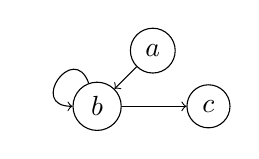
\begin{tikzpicture}[main/.style = {draw, circle}]
    \node[main] (1) {$a$};
    \node[main] (2) [below left of = 1] {$b$};
    \node[main] (3) [below right of = 1] {$c$};
    \draw[->] (1) -- (2);
    \draw[->] (2) -- (3);
    \draw[->] (2) to [out = 110, in=180, looseness = 4] (2);
\end{tikzpicture}
$$

Given a graph $G = (N,E)$, we define the \emph{out-degree} of a node $v$ to be the number of edges that have $v$ as its source: 
$$\mathsf{out}(v) := | \{e : e = (v,u) \text{ for some } u \in N \} | = | \{u : (v,u) \in E \} | $$
since there is at most one edge from $u$ to $v$. For instance, the out-degree of $b$ in $F$ is 2.

A \emph{(directed) walk} from $v_1$ to $v_n$ in a graph $G = (N,E)$ is a sequence of nodes $(v_1, \ldots, v_n)$ such that $(v_i, v_{i+1}) \in E$ for all $1 \leq i \leq n-1$. There is a trivial walk $(v)$ from each node $v$ to itself. A \emph{(directed) path} is a directed walk in which we do not traverse any node more than once. It turns out that any walk from $v_1$ to $v_n$ contains a path from $v_1$ to $v_n$. For example, in F we have paths $(a), (b), (c), (a,b), (b,c), (a,b,c)$. The walk $(a,b,b,c)$ is not a path.

The \emph{transitive closure} of a graph $G = (N, E)$ is defined to be the graph $\bar G = (N, P(E))$ whose nodes are $N$ and where $(u,v) \in P(E)$ iff there is a path from $u$ to $v$ in $G$.

\paragraph{Task} The aim is to implement
\begin{enumerate}
    \item a datatype \verb|Graph a| of graphs whose nodes are of type \verb|a|.
    \item a function \verb|outDegree :: a -> Graph a -> Int| which returns the outdegree of any node,
    \item a function \verb|isPath :: a -> a -> Graph a -> Bool| which return whether there is a path between two nodes,
    \item a function \verb|closeGraph :: Graph a -> Graph a| which returns the transitive closure of a graph.
\end{enumerate}

For this task, I suggest using \verb|Data.Set|. This module includes almost anything you would want to do with sets. Moreover,
\begin{enumerate}
    \item Implement \verb|Graph a| using \href{https://devtut.github.io/haskell/record-syntax.html#basic-syntax}{record syntax}. Its nodes should be a set of type \verb|a| and its edges a set of pairs \verb|(a,a)|.
    \item Write a function \verb|outNeighbors :: a -> Graph a -> Set a| which given a node $v$ and graph $G = (N,E)$ returns the set $\{u : (v,u) \in E \}$ of \emph{out-neighbors} of $v$. This will be useful later as well. Use \verb|outNeighbors| to compute the outdegree.
    \item This is the most complicated task. I suggest:
    \begin{enumerate}
        \item Write a function 
\begin{verbatim}
setPath :: (Eq a, Ord a) => Set a -> a 
            -> Set a -> Graph a -> Bool
\end{verbatim}
        which takes a starting set of nodes $S$, a target node $t$, a set of previously visited nodes $V$, and a graph $G$. \verb|setPath| should check if there is a path from some node in $S$ to $t$. The visited nodes are required to track our exploration of the graph. If $t \in S$ or $S = \emptyset$, we know the return value. Otherwise, perform the recursive step by calling \verb|setPath| with starting nodes $\mathtt{outNeighbors}(S) \setminus V$, and visited nodes $V \cup S$. The idea is that we move to the unvisited out-neighbors of $S$ and update our visited nodes to include $S$.
        \item Use \verb|setPath| to write \verb|isPath| as a special case. 
    \end{enumerate}
    \item Use \verb|isPath| to define the edges of the closure.
\end{enumerate}

\end{document}